\documentclass[a4paper,12pt]{report}
\usepackage{url}
\usepackage{enumitem}
\usepackage{palatino}
\usepackage[cmex10]{amsmath}
\usepackage{stmaryrd,amssymb}
\usepackage{graphicx}
\usepackage{amsfonts}
\usepackage{rotating}
\usepackage{listings}
\usepackage{xcolor}
\usepackage{url,boxedminipage,listings}
\usepackage{booktabs}
\usepackage{rotating}
\usepackage{array}
\usepackage{color,url,varioref,xcolor}
\usepackage{alltt,epsfig,comment}
\usepackage{supertabular,fancyhdr}
\usepackage{multirow}
\usepackage{url}
\usepackage{xspace}
\usepackage{dsfont}
\usepackage[english]{babel}
\usepackage{todonotes}

\usepackage{pdfpages}
\usepackage[font={footnotesize,sl}, labelfont=bf] {caption}

\usepackage{tikz}
\usetikzlibrary{arrows}
\usetikzlibrary{automata}
\usetikzlibrary{positioning}
\usetikzlibrary{er}

% HAS TO BE LAST PACKAGE:
\usepackage[pdftex,bookmarks=true,pageanchor=false]{hyperref}



% Eiffel Code Stuff
\lstset{language=OOSC2Eiffel,basicstyle=\ttfamily\small}
\definecolor{codebg}{rgb}{0.95,0.95,0.95}
\setlength{\headheight}{28pt}

% Inline Eiffel Code
\let\e\lstinline
% Eiffel Identifiers or expressions
\newcommand{\eid}[1]{\textsl{{\color[HTML]{000000} #1}}}
% Eiffel Class names
%\newcommand{\ecl}[1]{\textsl{{\color[HTML]{3333FF} #1}}}
\newcommand{\ecl}[1]{\textsl{{\color[HTML]{000000} #1}}}
% Eiffel Keywords
%\newcommand{\ekey}[1]{\textbf{{\color[HTML]{333399} #1}}}
\newcommand{\ekey}[1]{\textbf{{\color[HTML]{000000} #1}}}

\newcommand{\distance}[2]{\ensuremath{#1\leftrightarrow#2}}

\lstset{escapechar=\$}

%\newcommand{\blankpage}{
%\newpage
%\thispagestyle{empty}
%\mbox{}
%\newpage
%}


\title {ABEL Technical Documentation}
\author {
	\textbf{Roman Schmocker} \\
	\textbf{Reviewed by:} Marco Piccioni
}


\begin{document}

%\pagenumbering{roman}
%
\includepdf {../includes/title_page}
\maketitle

%\blankpage

%\section*{Abstract}

ABEL is an approach to wrap every existing persistence library under a simple and yet powerful API.
The programming interface of ABEL is completely transparent to the actual storage mechanism, and it supports the CRUD operations, transactions, and some advanced features like result filtering based on some criteria.

ABEL has a flexible framework that allows to adapt the API to basically any existing persistence solution.
The framework has a reusable object-relational mapper at its core and is open for extensions and customization.

%\blankpage

\tableofcontents


\pagenumbering{arabic}

\chapter{Introduction}
ABEL (A Better Eiffelstore Library) aims at providing a unified, easy to use object-oriented interface to different kinds of persistence stores, trying to be as back-end-agnostic as possible.

For the basic read and write operations of the API have a look at the ABEL tutorial. 

This is an introduction to the general architecture of ABEL.
%and some selected topics like the object-relational mapping layer or the main interfaces for the backend abstraction.

At the moment the supported back-ends are an in-memory database, MySQL, and SQLite. 
 
\chapter{Architecture overview}

The ABEL library can be split into a front-end and a back-end part.
The front-end provides the main API, which is completely agnostic of the actual storage engine, 
whereas the backend provides a framework and some implementations to adapt ABEL to a specific storage engine.
The boundary between backend and front-end can be drawn straight through the deferred class \lstinline!REPOSITORY!.

\section{Front-end}

If you've read the previous part of the documentation, then you should be quite familiar now with the front-end.
The main classes are:
 \begin{itemize}
  \item \lstinline!TRANSACTION!: Represents a transaction and can be used for read and write operations.
  \item \lstinline!QUERY!: Collects information like the Criteria, Projection and the type of the object to be retrieved (through its generic parameter).
  \item \lstinline!REPOSITORY!: Hides the actual storage mechanism, and can be used for read operations or for creating new transactions.
  \item \lstinline!CRITERION!: Its descendants provide a filtering function for retrieved objects, and it has features to generate a tree of criteria using the overloaded logical operators.
 \end{itemize}

You can see that the main objective of the front-end is to provide an easy to use, backend-agnostic API and to collect information which the backend needs.

% The class diagram provides an overview over the front-end.
% Note that this diagram only shows the most important classes and their relations.
% 
% \begin{figure} [h]
% \centering
% 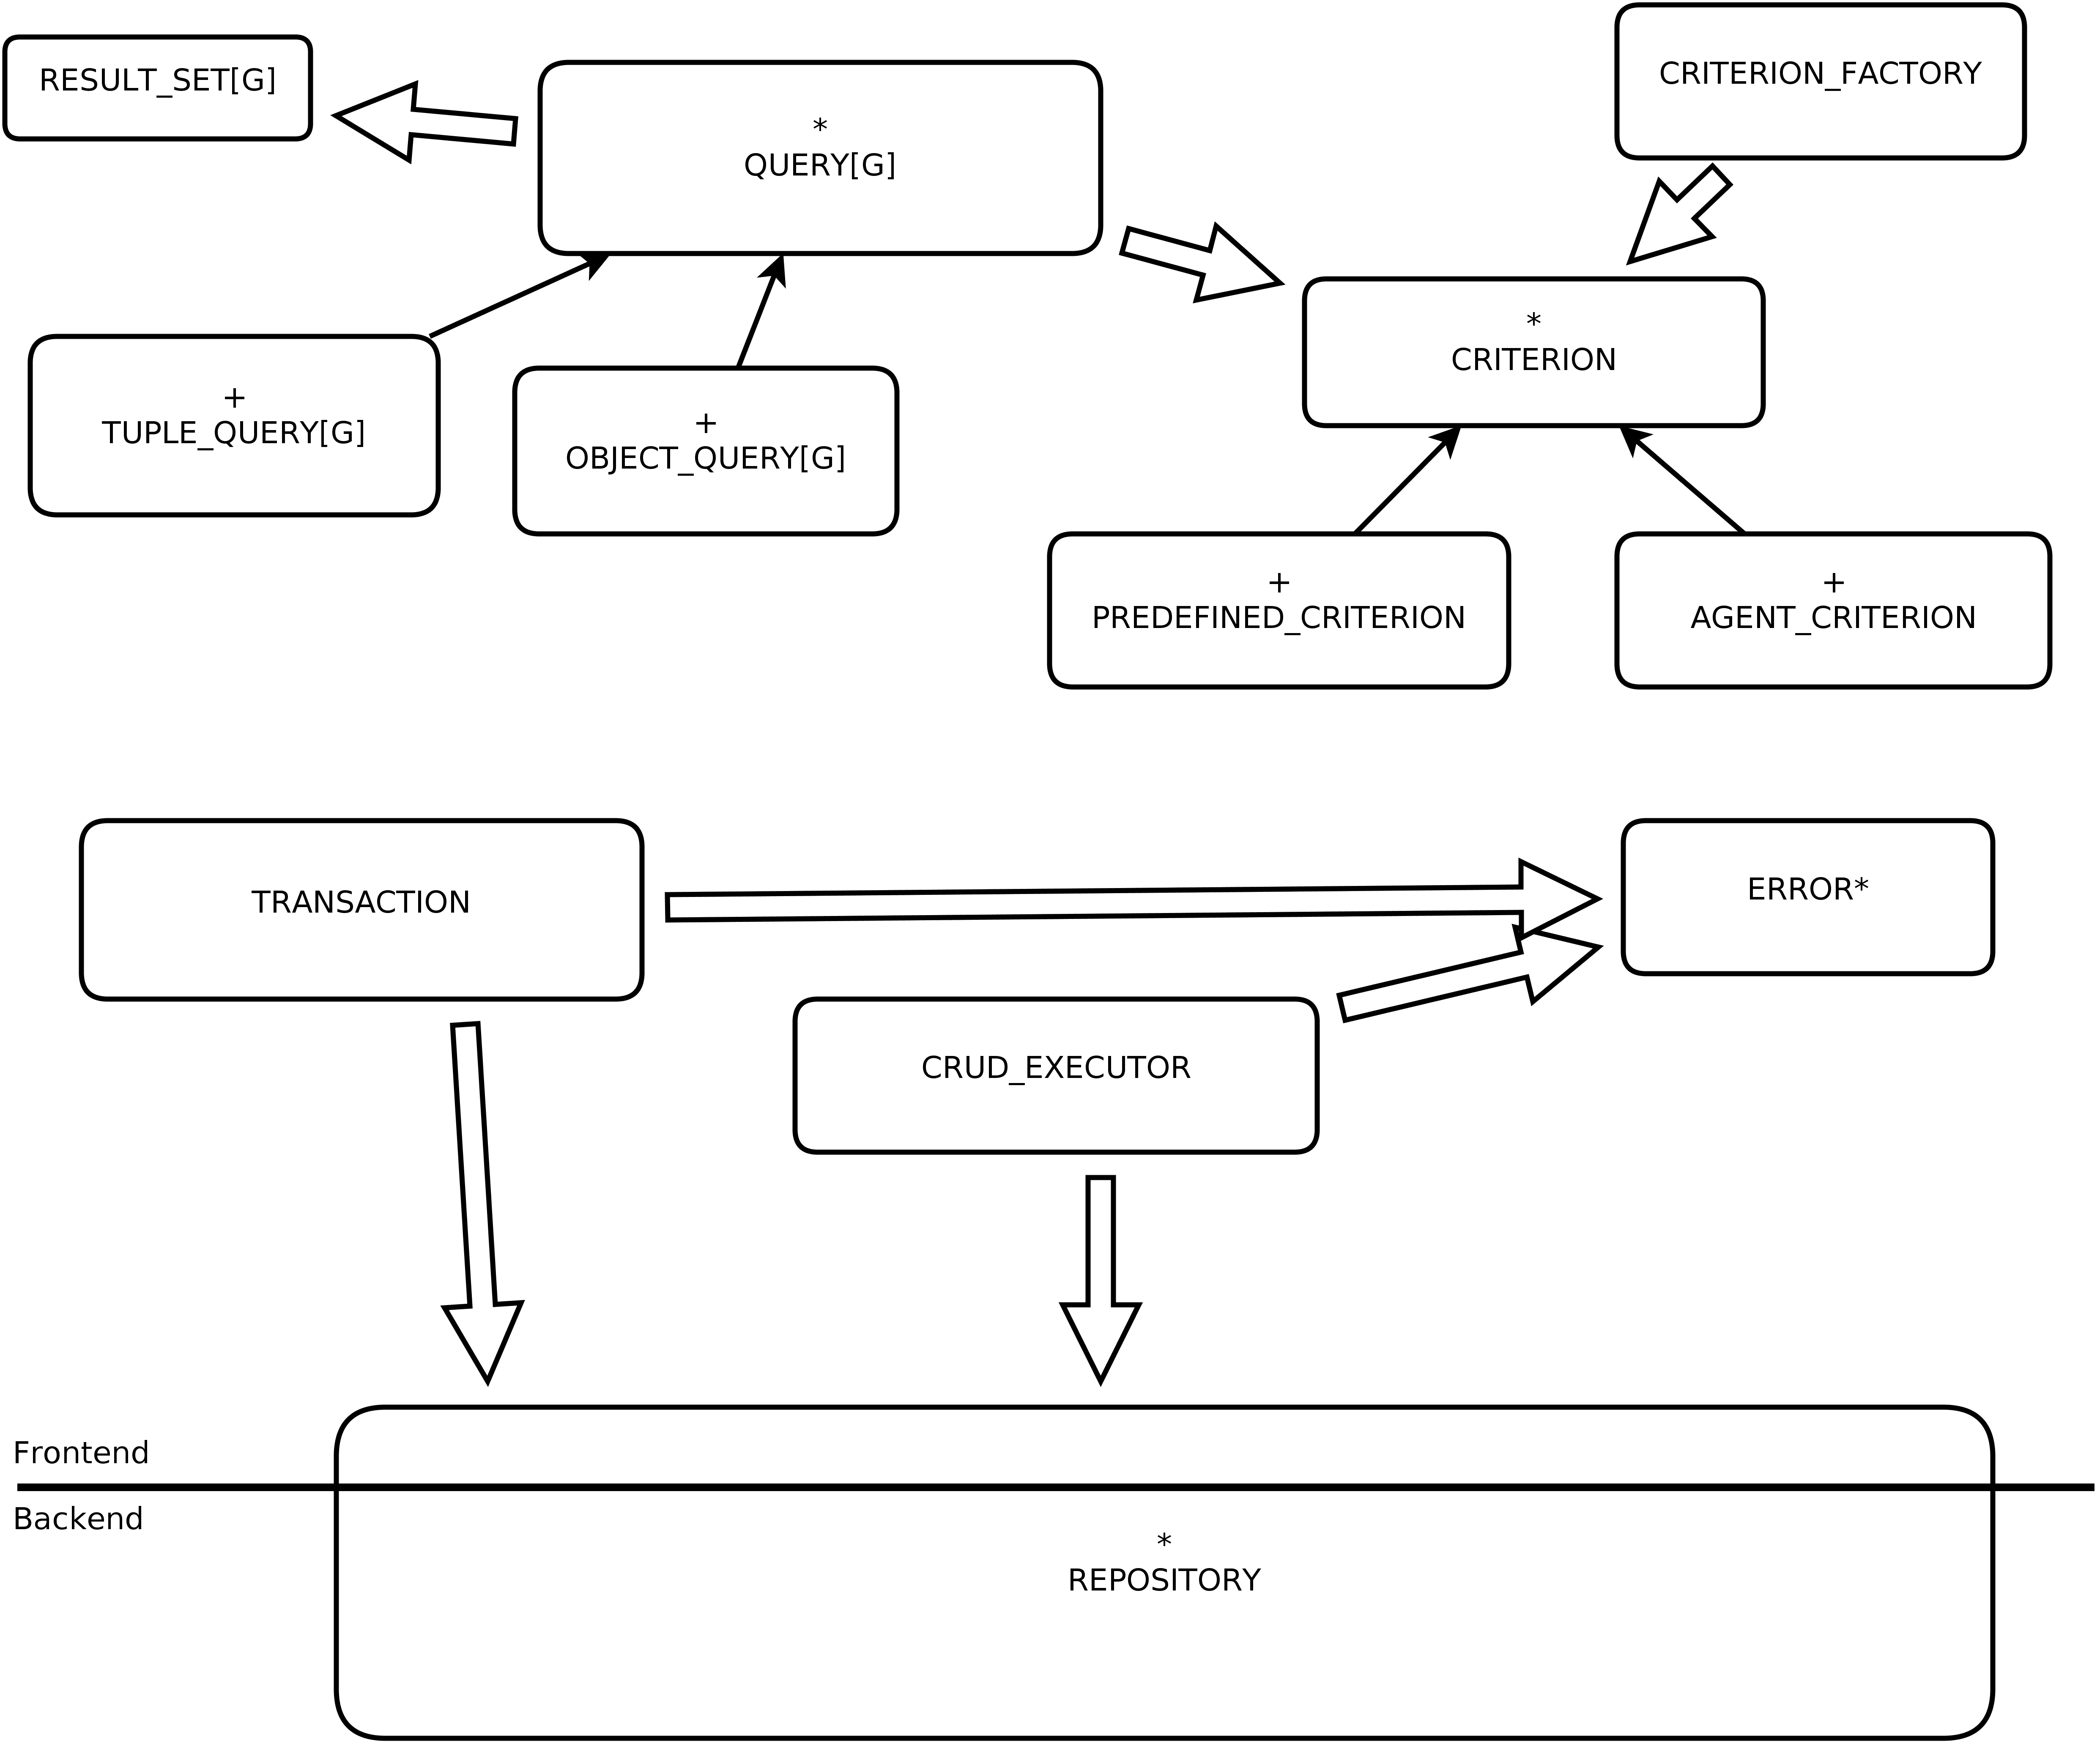
\includegraphics[trim= 0mm -10mm 0mm -10mm,clip, width = 13cm] {../includes/frontend.png}
% \caption{The main front-end classes and their relations.}
% \label{fig:front-end_classes}
% \end{figure}


\section{Back-end}

The front-end needs a repository which is specific to a persistence library, and the back-end part provides a framework to implement these repositories (in cluster \lstinline!framework!).

There are also some predefined repositories inside the back-end (cluster \lstinline!backends!), like the \lstinline!IN_MEMORY_BACKEND!.

\subsection{The framework layers}

The framework is built of several layers, with each layer being more specific to a persistence mechanism as it goes down.

The uppermost layer is the \lstinline!REPOSITORY! class. 
It provides a very high level of abstraction, as it deals with normal Eiffel objects that may reference a lot of other objects.

One level below you can find the object graph traversal layer.
It is responsible to take an object graph apart into its pieces and generate a more suitable representation for the next layer.
During retrieval this layer is responsible for reconstructing the object graph from the data.
%This layer is described more precisely in section ~\ref{section:ORM}.

On the next level there is the \lstinline!BACKEND! layer.
Its task is to map the objects, represented as string-value pairs in class \lstinline!BACKEND_OBJECT!, 
to a specific storage engine like a database with some table layout.

The lowest level of abstraction is only significant for databases that understand SQL. 
It provides a set of wrapper classes that hide connection details and error handling, and it has features to execute SQL and retrieve the result in a standardized way.

\subsection{Important data structures}

The key data structure is the \lstinline!OBJECT_IDENTIFICATION_MANAGER!.
It maintains a weak reference to every object that has been retrieved or inserted before, and it assigns a repository-wide unique number to such objects.
It is for example responsible for the fact that an update to a newly created object fails 
%in section ~\ref{subsection:recognize_objects}, ``Recognizing Objects.''

Another important data structure is the \lstinline!KEY_POID_TABLE!, which maps the object's \lstinline!object_identifier! to the primary key of the corresponding entry in the database.

\subsection{Transactions}

Every operation runs inside a transaction, and almost every part in the back-end is aware of transactions.
For example, the two important data structures described above have to provide some kind of rollback mechanism, and ideally all ACID %\todo{cite?} 
properties as well.

Another important task of transactions is error propagation within the back-end.
If for example an SQL statement fails because of some integrity constraint violation, then the database wrapper can set the error field in the current transaction instance and raise an exception.
As the exception propagates upwards, every layer in the back-end can do the appropriate steps to bring the library back in a consistent state, using the transaction with the error inside to decide on its actions.

% \subsection{Class diagram}
% 
% To visualize the whole structure, there is a class diagram that shows the most important classes and concepts of the back-end.
% 
% \begin{figure} [h]
% \centering
% 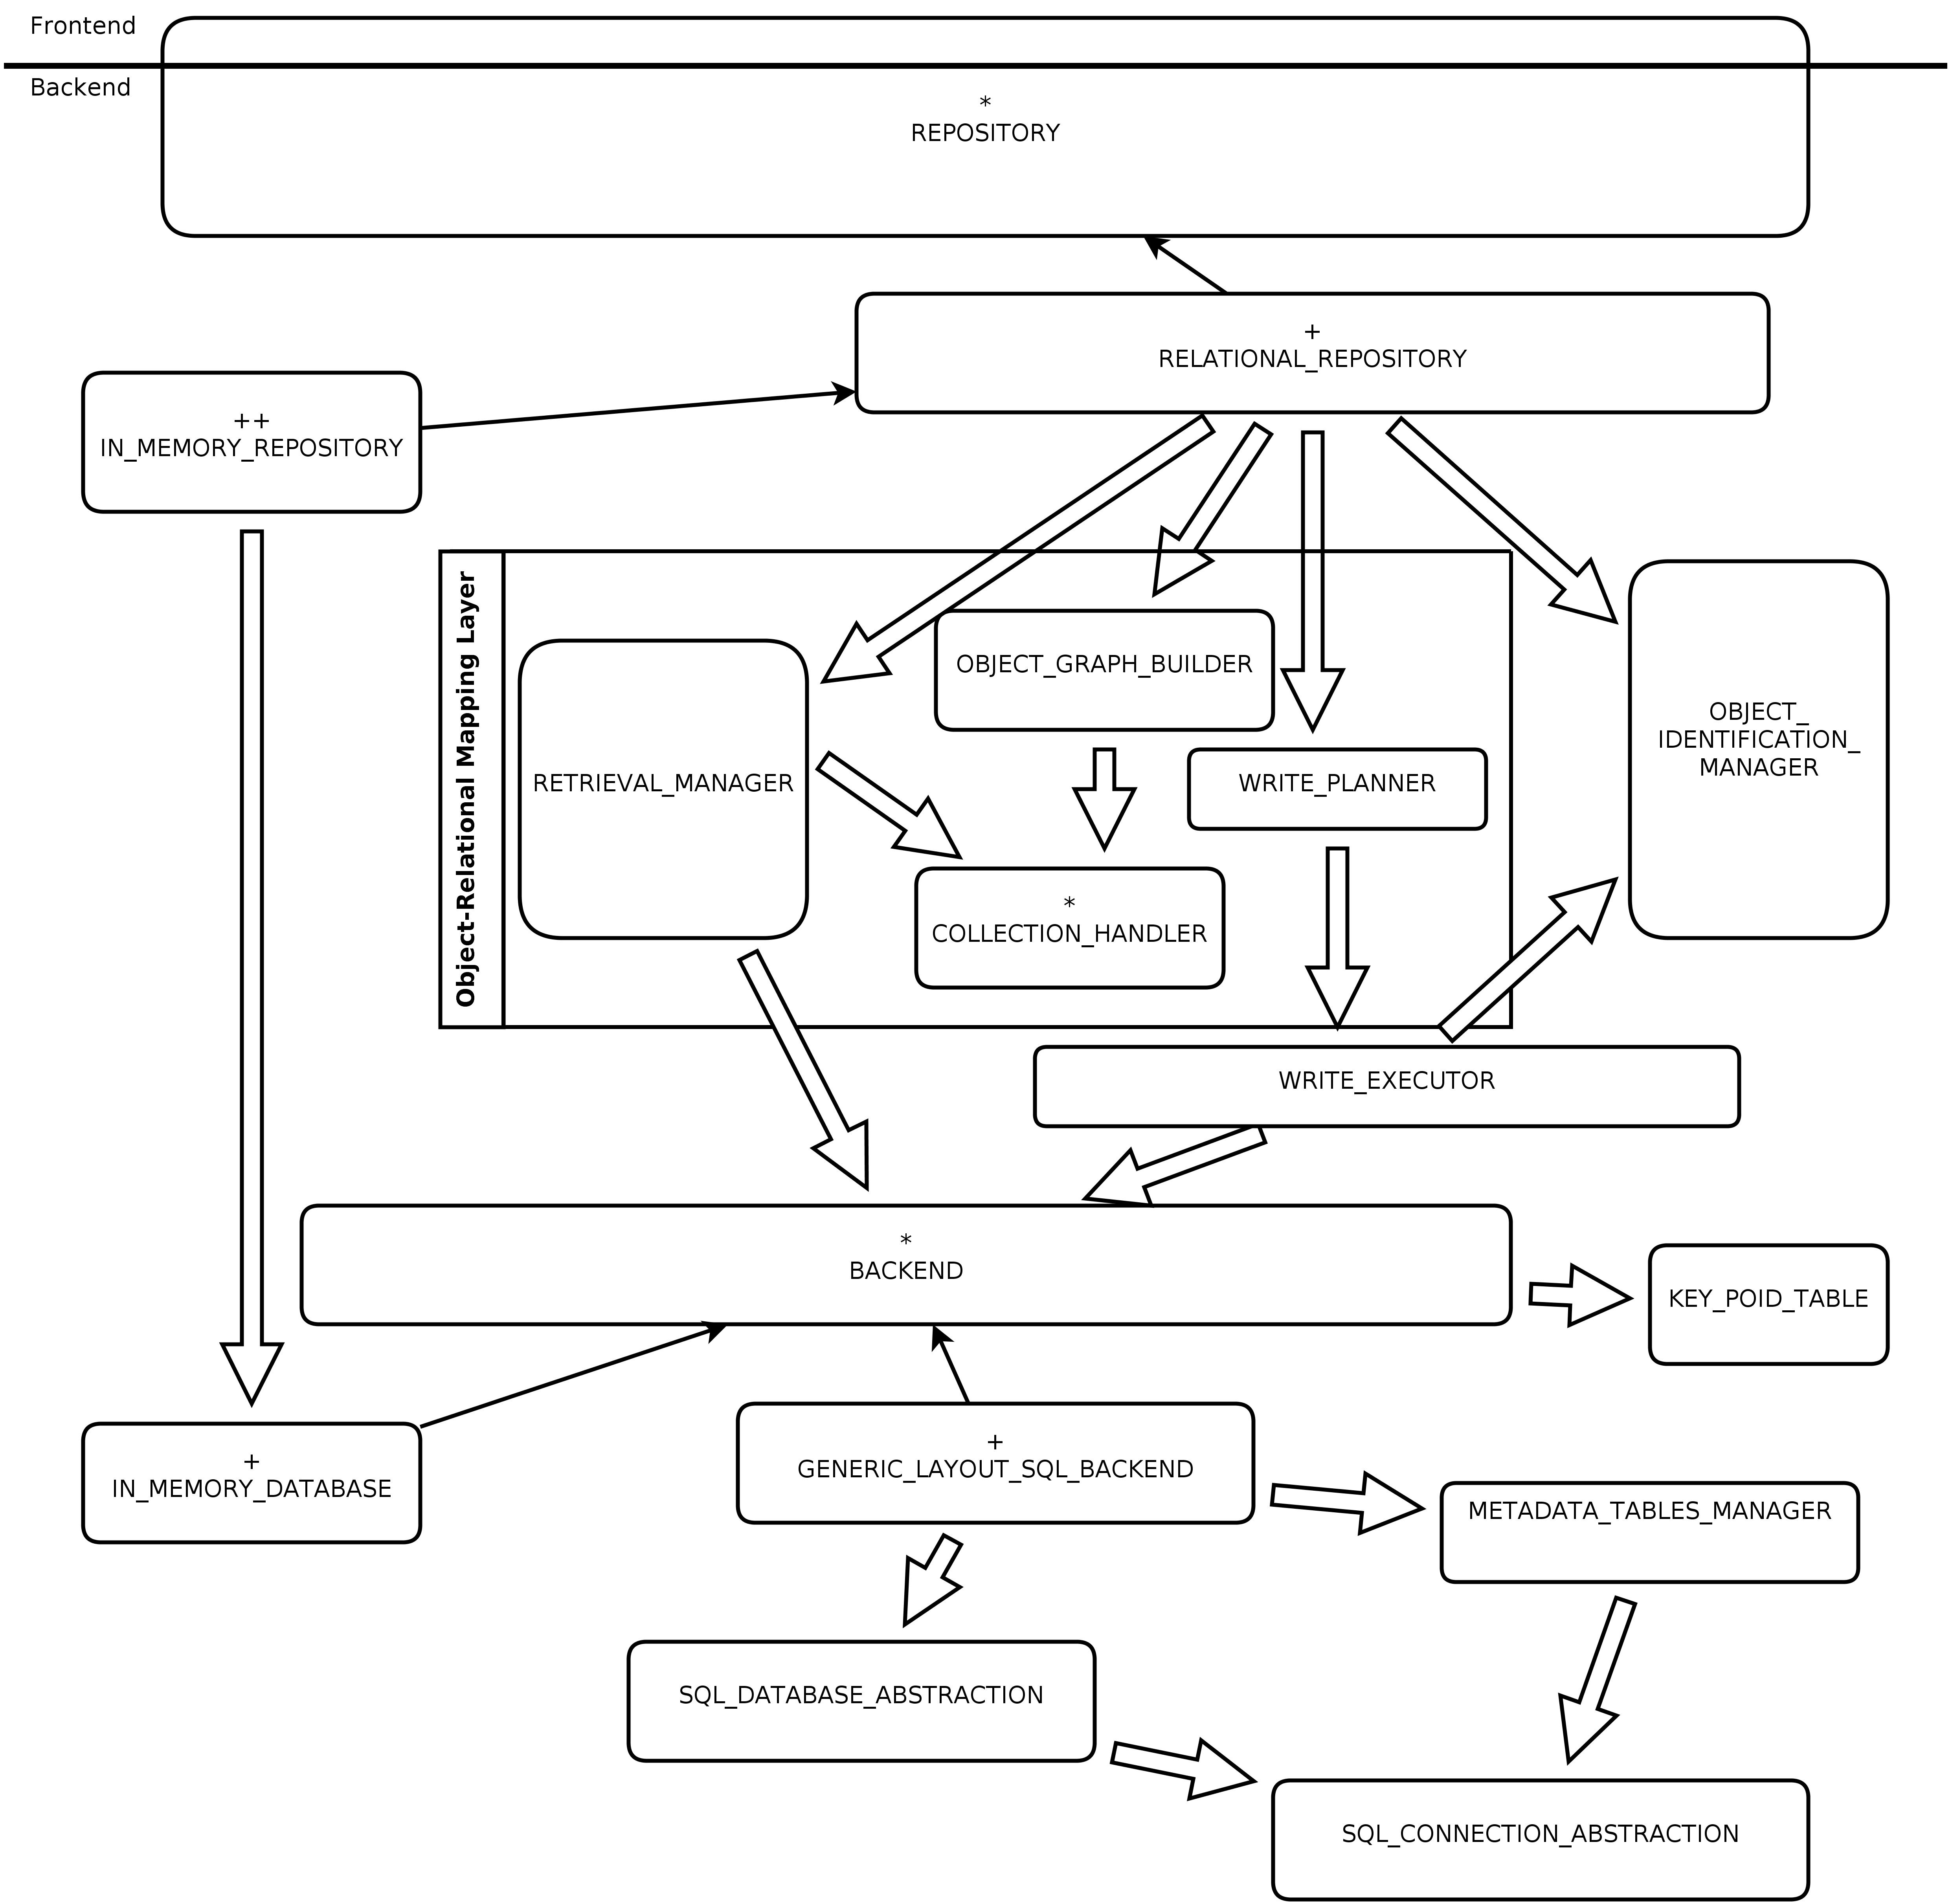
\includegraphics[trim= 0mm -10mm 0mm -10mm,clip, width = 13cm] {../includes/backend.png}
% \caption{The main back-end classes and their relations.}
% \label{fig:backend_classes}
% \end{figure}

% 
% \chapter{Object-relational Mapping}
% \label{section:ORM}
% 
% The object-relational mapping layer (abbreviated as ORM layer) lies between the \lstinline!REPOSITORY! and the \lstinline!BACKEND!.
% It consists of four main classes doing the actual work, and a set of helper classes to represent an object graph.
% 
% All helper classes are in \lstinline!framework/object_graph_representation!.
% Besides representation of an object graph, they are also used to describe a write operation in the \lstinline!BACKEND!.
% The most important ones are:
% 
% \begin{itemize}
%  \item \lstinline!BASIC_ATTRIBUTE_PART! represents an object of a basic type
%  \item \lstinline!COLLECTION_PART! represents a collection, for example an instance of \lstinline!SPECIAL!
%  \item \lstinline!SINGLE_OBJECT_PART!: represets an Eiffel object that is neither a basic type nor a collection
% \end{itemize}
% 
% All helper classes inherit from \lstinline!OBJECT_GRAPH_PART!. 
% They have a built\-in iteration cursor, and they share the concept of a dependency:
% If an object graph part $X$ is dependent on another part $Y$, then it means for example that $Y$ has to be inserted first, because $X$ needs $Y$'s primary key as a foreign key in the database.
% 
% The four classes listed here are the ones that do the actual work:
% 
% \begin{itemize}
%  \item The \lstinline!OBJECT_GRAPH_BUILDER! is responsible to create the explicit object graph representation.
%  \item The \lstinline!WRITE_PLANNER! is responsible to generate a total order on all write operations, taking care of the dependency issues.
%  \item The \lstinline!RETRIEVAL_MANAGER! builds objects from the parts that it gets from the backend, and takes care that the complete object graph gets loaded.
%  \item The \lstinline!COLLECTION_HANDLER!, or rather its descendants, add collection handling support to the basic ORM layer. 
%  You need at least one handler for \lstinline!SPECIAL!, but you can add handlers for other collections as well.
% \end{itemize}
% 
% The graph visualizes the process and shows the intermediate representation of data in the object-relational mapping layer.
% You can see there that the object writing part is a bit more complex than the reading part, because of the dependency issue.
% 
% 
% \begin{figure} [h!]
% \centering
% 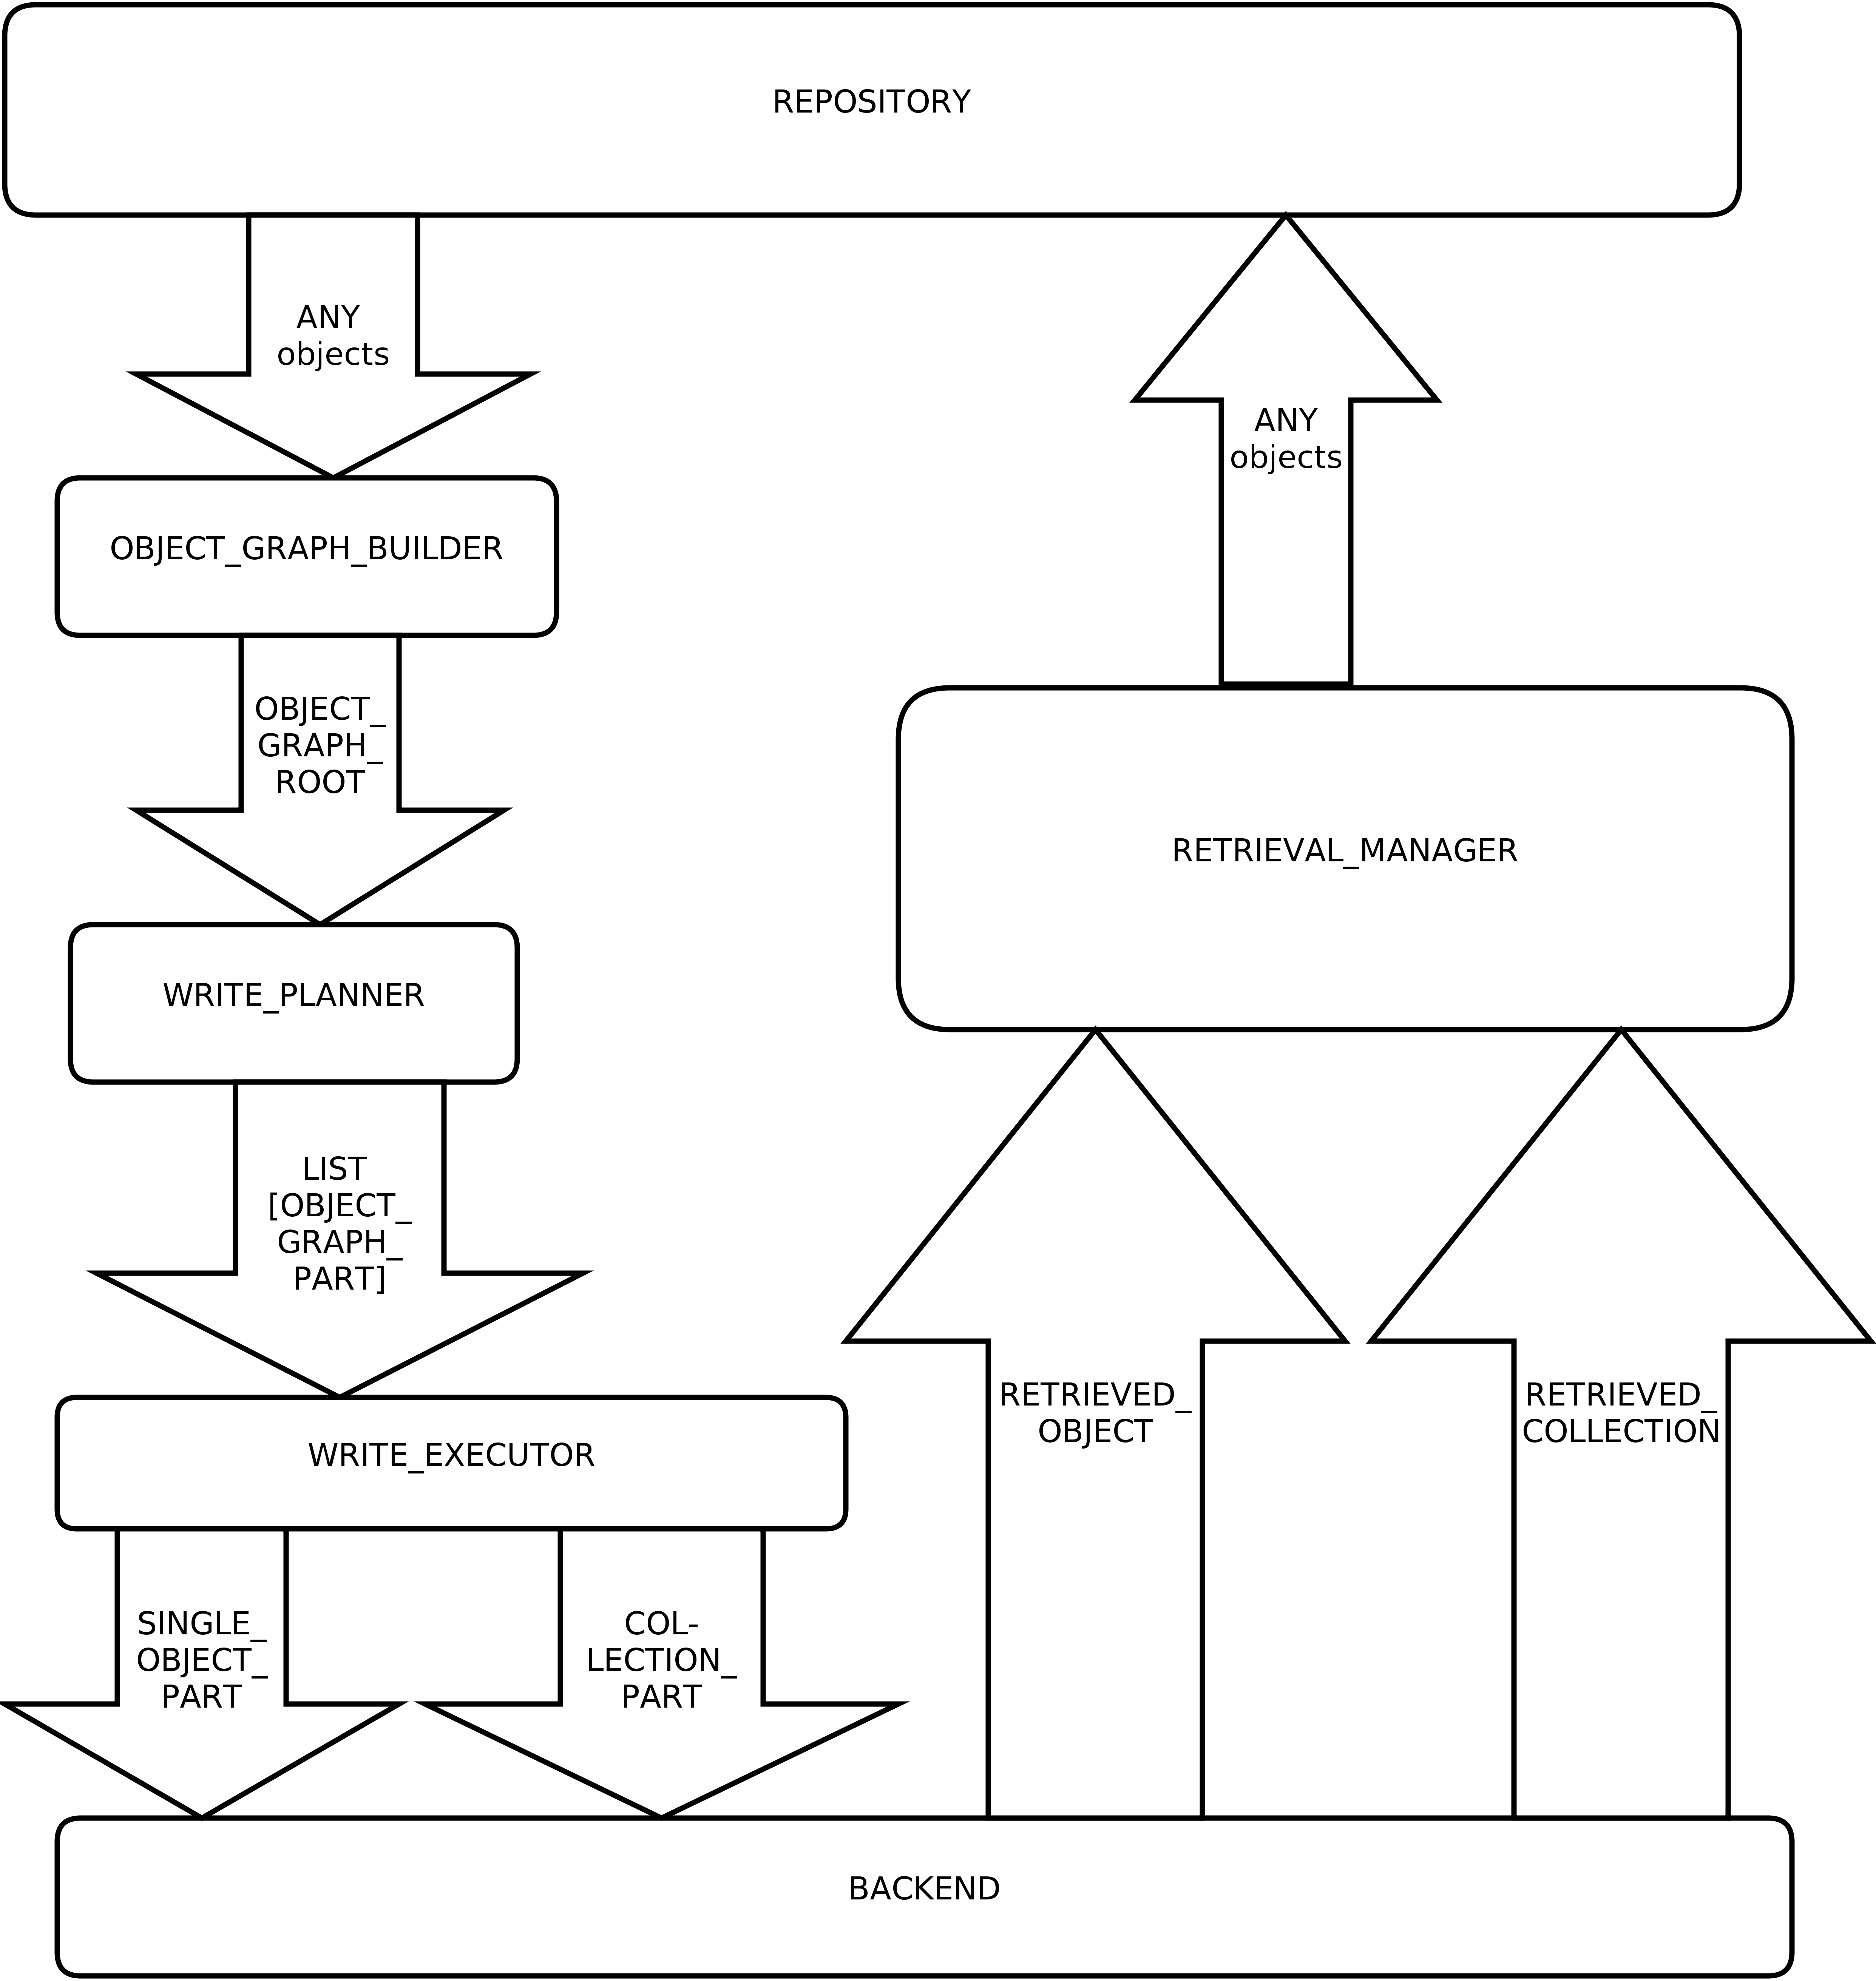
\includegraphics[trim= 0mm -10mm 0mm -10mm,clip, width = 13cm] {../includes/dataflow.png}
% \caption{The different intermediate representations of data.}
% \label{fig:intermediate_data_orm}
% \end{figure}
% 
% 
% 
% \section{Collection handling}
% 
% You can extend the ORM algorithm to include collections. A collection is usually mapped differently from a normal object in the backend, e.g. through an M:N-relation table.
% You need at least one handler for \lstinline!SPECIAL!, because of its peculiarity that it doesn't have a fixed amount of fields, but you can include any other collection, like a \lstinline!LIST! or an \lstinline!ARRAY!.
% 
% There are two types of collections you can create within a handler. 
% The \lstinline!RELATIONAL_COLLECTION! is intended for a case when you have a typical database layout, 
% with tables for every specific class and relations stored either within the table of the referenced object (1:N-Relations) or inside their own table (M:N-Relations).
% 
% The \lstinline!OBJECT_COLLECTION! is intended for a scenario where you store collections in a separate table, 
% having their own primary key, and with the collection owner using this key as a foreign key.
% 
% The following diagrams shows an example entity-relationship model for each type of collection:
% 
% \begin{figure} [h!]
% \centering
% \begin{tikzpicture}[node distance=2.5cm, auto]
%  
% \node[entity] (1) {$Professor$};
% \node[relationship] (2) [right of= 1] {$gives$};
% \node[entity] (3) [right of = 2] {$LectureList$};
% \node[relationship] (4) [right of= 3] {$has$};
% \node[entity] (5) [right of=4] {$Lecture$};
% 
% 
%   \path
%     (1) edge node {$1$} (2)
%     (2) edge node {$1$} (3)
%     (3) edge node {$1$} (4)
%     (4) edge node {$N$} (5);
%  
% \end{tikzpicture}
% %\includegraphics[trim= 0mm -10mm 0mm -10mm,clip, width = 13cm] {collection_er1.png}
% \caption{An ER-model where an OBJECT\_COLLECTION can be used.}
% \label{fig:object_collection_er}
% \end{figure}
% 
% \begin{figure} [h!]
% \centering
% \begin{tikzpicture}[node distance=3.5cm, auto]
%  
% \node[entity] (1) {$Student$};
% \node[relationship] (2) [right of= 1] {$attend$};
% \node[entity] (3) [right of = 2] {$Lecture$};
% 
%   \path
%     (1) edge node {$M$} (2)
%     (2) edge node {$N$} (3);
%  
% \end{tikzpicture}
% %\includegraphics[trim= 0mm -10mm 0mm -10mm,clip, width = 13cm] {collection_er2.png}
% \caption{An ER-model where a RELATIONAL\_COLLECTION with M:N mapping can be used.}
% \label{fig:relational_m_n_er}
% \end{figure}
% 
% \begin{figure} [h!]
% \centering
% \begin{tikzpicture}[node distance=3.5cm, auto]
%  
% \node[entity] (1) {$Professor$};
% \node[relationship] (2) [right of= 1] {$gives$};
% \node[entity] (3) [right of = 2] {$Lecture$};
% 
%   \path
%     (1) edge node {$1$} (2)
%     (2) edge node {$N$} (3);
%  
% \end{tikzpicture}
% %\includegraphics[trim= 0mm -10mm 0mm -10mm,clip, width = 13cm] {collection_er3.png}
% \caption{An ER-model where a RELATIONAL\_COLLECTION with 1:N mapping can be used.}
% \label{fig:relational_1_n_er}
% \end{figure}
% 
% 
% Note that the choice of the collection part has an effect in the object-re\-la\-tio\-nal mapping layer already:
% \begin{itemize}
%  \item \lstinline!OBJECT_COLLECTION!s are handled like a \lstinline!SINGLE_OBJECT_PART!: The owner of the collection object depends on the collection, and the collection depends on all items that it references.
%  \item A \lstinline!RELATIONAL_COLLECTION! in an M:N mapping mode depends on both the collection owner and all items that it references, but the owner does not depend on its collection.
%  This comes from the fact that you need both a foreign key of the owner and the collection item to insert a single row in an M:N-relation table.
%  \item A \lstinline!RELATIONAL_COLLECTION! in a 1:N mapping mode actually isn't forwarded to the backend at all. 
%  Instead, each item in the collection gets a new dependency to the collection owner.
%  Again, this comes from the normal practice in database layouts for 1:N relations.
% \end{itemize}
% 
% 
% If you use one of the predefined backends, you usually don't have to care about collection handlers.
% They get important however if you want to adapt ABEL to a custom database layout, as you can see in section ~\ref{subsection:specific_adaption}.
% 
% Please note that the framework itself does not provide any collection handler, and inserting a \lstinline!SPECIAL! object without setting an appropriate handler will result in a runtime crash.
% However, there is a handler for \lstinline!SPECIAL! shipped with the predefined backends, which is used for example by the \lstinline!IN_MEMORY_REPOSITORY!.
% 
% \section{Object graph settings}
% \label{subsection:obect_graph_settings}
% 
% First, let's define the object graph more exactly, using graph theory.
% An object corresponds to a vertex in the graph, and a reference is a directed edge.
% 
% The (global) object graph is the web of objects and references as it is currently in main memory.
% 
% An object $Y$ can be $reached$ from another object $X$ if there is a path between $X$ and $Y$, i.e. $Y$ is in the transitive closure of $X$.
% 
% The object graph of an object $X$ is the induced subgraph of the global object graph that contains all vertices that can be reached from $X$.
% 
% The $level$ of an object $Y$ in the object graph of $X$ is the length of the shortest path from $X$ to $Y$.
% 
% Using these definitions we can now describe how ABEL handles object graphs, and how you can tweak the default settings to increase performance.
% 
% Every operation in ABEL has its own $depth$ parameter, which is defined in \lstinline!OBJECT_GRAPH_SETTINGS!.
% An operation will only handle an object when the following condition holds:
% 
% \begin{center}
%  $ level(object) < depth $ 
% \end{center}
% 
% Now let's put this in a context:
% You already know that the insert and retrieve features handle the complete object graph of an object. 
% In fact, the depth for both functions is $Infinity$ by default.
% 
% On the other hand, the update or delete operations only handle the first object they get, and don't care about the object graph.
% Their depth is defined as exactly $1$, which means that only an object with a level of $0$ satisfies the condition above.
% The only object with level $0$ is in fact the root object of an object graph.
% 
% To fully understand the behaviour of ABEL, we also have to look at what happens when the algorithm reaches the ``last'' object, i.e. when the condition $level + 1 = depth$ holds.
% In that case the object with all basic attributes gets inserted/updated, but references only get written if the referenced object is already persistent.
% If it isn't persistent, then in a later retrieval operation the reference will be Void.
% 
% You can change the depth parameter of the individual operations in \lstinline!REPOSITORY.default_object_graph!. 
% Please keep in mind that this is a dangerous operation, because a partially loaded object will contain Void references even in a void-safe environment and may also violate its invariant.
% 
% Apart from the depth, there are some other settings as well, i.e. what ABEL should do if it finds an already persistent object along the object graph of a new object to insert, or vice versa.

\chapter{Backend abstraction}

The framework provides some very flexible interfaces to be able to support many different storage engines. 
The three main levels of abstraction are the \lstinline!REPOSITORY!, the \lstinline!BACKEND! and the database wrapper classes.

\section{REPOSITORY}

The deferred class \lstinline!REPOSITORY! provides the highest level of abstraction, as it deals with raw Eiffel objects including their complete object graph.
It provides a good interface to wrap a persistence mechanism that provides a similarly high level of abstraction, like for example db4o \cite{db4o}.

The \lstinline!DEFAULT_REPOSITORY! is the main implementation of this interface.
It uses the ORM layer and a \lstinline!BACKEND! and is therefore the default repository for persistence libraries which are wrapped through \lstinline!BACKEND!.

\section{BACKEND}

Another important interface is the deferred class \lstinline!BACKEND!.
This layer only deals with \lstinline!BACKEND_OBJECT! or \lstinline!BACKEND_COLLECTION!.
It is responsible to map them to the actual persistence mechanism which is usually a specific layout in a database.

Its use however is not restricted to relational databases.
The predefined \lstinline!IN_MEMORY_DATABASE! backend for example implements this interface to provide a fake storage engine useful for testing, and it is planned to wrap the serialization libraries using this abstraction.

\section{Database wrapper}


The last layer of abstraction is a set of wrappers to a database. 
It consists of three deferred classes: 
\begin{itemize}
 \item The \lstinline!SQL_DATABASE! represents a database. Its main task is to acquire or release a \lstinline!SQL_CONNECTION!.
 \item The \lstinline!SQL_CONNECTION! represents a single connection. 
It has to forward SQL statements to the database and represent the result in an iteration cursor of \lstinline!SQL_ROW!s.
Another important task is to map database specific error messages to ABEL \lstinline!ERROR! instances.
  \item The \lstinline!SQL_ROW! represents a single row in the result of an SQL query.
\end{itemize}

The wrapper is very useful if you want to easily swap e.g. from a MySQL database to SQLite.
However, keep in mind that the abstraction is not perfect. 
For example, the wrapper doesn't care about the different SQL variations as it just forwards the statements to the database.

To overcome this problem, you can put all SQL statements in your implementation of \lstinline!BACKEND! into a separate class, and generally stick to standard SQL as much as possible.


% \chapter{Extensions}
% 
% Due to its flexible abstraction mechanism, you can easily extend ABEL with features like client-side transaction management or ESCHER \cite {PiccioniOriolMeyer12} integration.
% 
% The general pattern on how to do this is quite simple: 
% You can implement the extension in a class that inherits from \lstinline!BACKEND! and forwards all calls to another \lstinline!BACKEND! that does the actual storage.
% Then the extension can do some processing on the intermediate result.
% That way you can add:
% 
% \begin{itemize}
%  \item Filter support for some non-persistent attributes by removing them from the \lstinline!OBJECT_GRAPH_PART! during a write, and adding a default value during retrieval.
%  \item ESCHER support by checking on the version attribute during a retrieval and calling the conversion function if necessary.
%  \item Client-side transaction management by using a multiversion concurrency control mechanism and delaying write operations until you can definitely commit.
%  \item Caching of objects by using an \lstinline!IN_MEMORY_DATABASE! alongside the actual backend.
%  \item An instance that does correctness checks, e.g. by routing the calls to two different backends and comparing if the results are the same.
%  \item Anything else you can imagine...
% \end{itemize}
% 
% The nice thing is that you can add such extensions without adding much complexity to the core of ABEL, and it works for all possible implementations of \lstinline!BACKEND! at once.


\chapter{Database adaption}

The \lstinline!BACKEND! interface allows to adapt the framework to many database layouts.
Shipped with the library is a backend that uses a generic database layout which can handle every type of object.
It is explained in the next section.

% But you can also adapt ABEL to your very own private database layout.
% An example on how to do this is shown in section ~\ref{subsection:specific_adaption}.

\section{The generic layout backend}

The database layout is based upon metadata of the class. 
It is very flexible and allows for any type of objects to be inserted.
The layout is a modified version from the suggestion in Scott W. Ambler's article ``Mapping Objects to Relational Databases'' \cite{AmblerORM}.

\begin{figure} [!ht]
\centering
\begin{tikzpicture}[node distance=3.5cm, auto]

\tikzstyle{every attribute} = [node distance = 2cm]


\node[entity] (1) [style=double] {$ps\_value$};
\node[relationship] (2) [style=double, right of= 1] {$attributeid$};
\node[entity] (3) [right of = 2] {$ps\_attribute$};
\node[relationship] (4) [above of = 3, node distance = 2.5cm] {$classid$};
\node[entity] (5) [above of = 4, node distance = 2.5cm] {$ps\_class$};

\node[attribute] (6) [above right of=1] {$\underline{objectid}$} edge (1);
\node[attribute] (7) [above left of=1] {$value$} edge (1);

\node[attribute] (8) [below left of=3] {$\underline{attributeid}$} edge (3);
\node[attribute] (9) [below right of=3] {$name$} edge (3);

\node[attribute] (10) [left of=5, node distance = 2.5cm] {$\underline{classid}$} edge (5);
\node[attribute] (11) [below left of=5] {$name$} edge (5);


  \path
    (1) edge[style=double] node {$1$} (2)
    (2) edge node {$N$} (3)
    (3) edge node {$1$} (4)
    (4) edge node {$N$} (5);
\end{tikzpicture}
\caption{The ER-Model of the generic database layout.}
\label{fig:er_model_generic_layout}
\end{figure}

The ER-model in figure~\ref{fig:er_model_generic_layout} is in fact a simplified view. 
The real model uses another relationship between value and class to determine the runtime type of a value, which is required in some special cases.

The backend located in \lstinline!backends/generic_database_layout! maps Eiffel objects to this database layout.

It is split into three classes:
\begin{itemize}
 \item The \lstinline!METADATA_TABLES_MANAGER! is responsible to read and write tables \lstinline!ps_class! and \lstinline!ps_attribute!.
 \item The \lstinline!GENERIC_LAYOUT_SQL_BACKEND! is responsible to write and read the \lstinline!ps_value! table. It is an implementation of \lstinline!BACKEND!.
 \item The \lstinline!GENERIC_LAYOUT_SQL_STRINGS! collects all SQL statements. Its descendants adapt the statements to a specific database if there is an incompatibility.
\end{itemize}

The functionality of the metadata table manager is quite easy:
It just caches table \lstinline!ps_class! and \lstinline!ps_attribute! in memory and provides features to get the primary key of an attribute or a class.
If the class is not present in the database, then it will insert it and return the new primary key.

Using the table manager, the \lstinline!GENERIC_LAYOUT_SQL_BACKEND! has all information to perform a write operation:
The attribute value inside the \lstinline!BACKEND_OBJECT!, the attribute foreign key which is stored inside the class \lstinline!METADATA_TABLES_MANAGER!, 
and the object primary key which is part of the \lstinline!BACKEND_OBJECT! as well.

The retrieval operation is similar.
First, the backend gets all attribute primary keys of a specific class from the table manager, and then it executes an SQL query to retrieve all values whose attribute foreign keys match the ones retrieved before.
The backend does also sort the result by the object primary key, such that attributes of the same object are grouped together.


% \section{Adaption to a custom database layout}
% \label{subsection:specific_adaption}
% 
% Adapting ABEL to a custom database layout needs two steps:
%  \begin{itemize}
%   \item Implement a \lstinline!BACKEND! for your layout
%   \item Implement \lstinline!COLLECTION_HANDLERS! for all collections that need to be mapped
%  \end{itemize}
% 
% Let's consider a very simple example with only two classes:
% 
% \begin{lstlisting}[language=OOSC2Eiffel, captionpos=b, caption={Example classes}, label={lst:example_application}]
% class
% 	PERSON
% 
% feature
% 	name:STRING
% 		-- Name of 'Current'
% 	items_owned: LINKED_LIST [ITEM]
% 		-- Items owned by 'Current'
% end
% 
% 
% class 
% 	ITEM
% 
% feature
% 	value:INTEGER
% 		-- The value of 'Current'
% end
% \end{lstlisting}
% 
% In the database, there is table \lstinline!Person! with columns \lstinline!primary_key! and \lstinline!name!, 
% and table \lstinline!Item! with columns \lstinline!primary_key!, \lstinline!item!, and a foreign key \lstinline!owner! to table \lstinline!Person!.
% 
% 
% \begin{figure} [h!]
% \centering
% \begin{tikzpicture}[node distance=3.5cm, auto]
% 
% \tikzstyle{every attribute} = [node distance = 2cm]
% 
% 
% \node[entity] (1) {$Person$};
% \node[relationship] (2) [right of= 1] {$owner$};
% \node[entity] (3) [right of = 2] {$Item$};
% 
% \node[attribute] (6) [above left of=1] {$\underline{primary\_key}$} edge (1);
% \node[attribute] (7) [below left of=1] {$name$} edge (1);
% 
% \node[attribute] (8) [above right of=3] {$\underline{primary\_key}$} edge (3);
% \node[attribute] (9) [below right of=3] {$value$} edge (3);
% 
%   \path
%     (1) edge node {$1$} (2)
%     (2) edge node {$N$} (3);
% \end{tikzpicture}
% \caption{The example ER-Model.}
% \label{fig:er_model_example}
% \end{figure}
% %\todo{ER-Model}
% 
% In this setup, you only need a collection handler for \lstinline!LINKED_LIST!.
% All \lstinline!LINKED_LIST! instances are relationally mapped in 1:M mode, therefore, the implementation of the (only) collection handler is very simple:
% 
% \begin{lstlisting}[language=OOSC2Eiffel, captionpos=b, caption={The collection handler for LINKED\_LIST}, label={lst:my_linked_list_collection_handler}]
% class 
% 	LINKED_LIST_HANDLER
% inherit
% 	PS_COLLECTION_HANDLER [LINKED_LIST [detachable ANY]]
% feature
% 
% 	is_relationally_mapped (collection, owner_type: PS_TYPE_METADATA):BOOLEAN
% 		-- Is `collection' mapped as a 1:N or M:N - Relation?
% 		do
% 			Result:= True
% 		end
% 
% 	is_mapped_as_1_to_N (collection, owner_type: PS_TYPE_METADATA):BOOLEAN
% 		-- Is `collection' mapped as a 1:N - Relation?
% 		do
% 			Result:= True
% 		end
% 
% 	build_relational_collection (collection_type: PS_TYPE_METADATA; objects: LIST[detachable ANY]): LINKED_LIST[detachable ANY]
% 		-- Build a new LINKED_LIST
% 		do
% 			create Result.make
% 			Result.append (objects)
% 		end
% 
% end
% \end{lstlisting}
% 
% 
% The implementation of \lstinline!BACKEND! is quite straightforward as well.
% You just have to distinguish between \lstinline!PERSON! and \lstinline!ITEM! objects and insert them in the corresponding table.
% 
% Please remember that the object-rlational mapping layer adds an attribute with name \lstinline!items_owned! to the \lstinline!ITEM! object, which is the default behaviour for 1:N relations.
% This especially means that you don't need to implement the write operations for relational collections.
% 
% The following code listing shows the insert feature in pseudocode:
% 
% \begin{lstlisting}[language=OOSC2Eiffel, captionpos=b, caption={The collection handler for LINKED\_LIST}, label={lst:my_backend_adaption}]
% class 
% 	MY_SIMPLE_BACKEND
% inherit
% 	PS_BACKEND
% feature
% 
% 	insert (object:PS_SINGLE_OBJECT_PART; tx:PS_TRANSACTION)
% 		-- Inserts the object into the database
% 		do
% 			if object is a PERSON object then
% 				database.execute_sql ("INSERT INTO person (name) VALUES " + object.attribute_value ("name"))
% 				key_mapper.add_entry (object, database.execute_sql ("Get autoincremented primary key of Person")
% 			else
% 				-- The ORM layer added `items_owned' to ITEM
% 				foreign_key:= key_mapper.primary_key_of (object.get_value ("items_owned"))
% 				database.execute_sql ("INSERT INTO item (value, owner) VALUES " + object.attribute_value ("value") + foreign_key)
% 				key_mapper.add_entry (object, database.execute_sql("Get autoincremented primary key of Item")
% 			end
% 		end
% 
% 	key_mapper: PS_KEY_POID_TABLE
% 		-- Maps object identifiers to primary keys
% end
% \end{lstlisting}
% 
% During a retrieval operation, you similarly have to select your values from the correct table.
% Please note that you have to implement the \lstinline!retrieve_relational_collection! feature here.


%\section{Tuning performance}

%Performance rather belongs to the future work section...


%\subsubsection{Performance remarks}

%ABEL will try to let the backend do as much of the filtering as is possible, to reduce the overhead of e.g. network communication or building unnecessary objects.
%This especially means that ABEL will compile predefined queries to SQL if you have a relational database as a backend. 
%However, if there is an agent criterion OR-ed to a predefined criterion, the test can not be made in the database because you might get false negatives.
%Therefore, to have optimal performance, you should consider the following points:

%\begin{itemize}
%\item Try not to use agent criteria if you have a relational database backend.
%\item Try not to use OR on agent criteria.
%\item Try to keep OR-ed agent criteria as deep down the tree as possible (as the above OR-node defaults to true and thus is not checked for in the backend)
%\end{itemize}


\begin{flushleft}
 
{{{
\bibliographystyle {plain}
\bibliography {./references}
}}}
\end{flushleft}
\end{document}